\begin{wrapfigure}{t!}{0.5\textwidth}
	%\begin{figure}
	\centering
	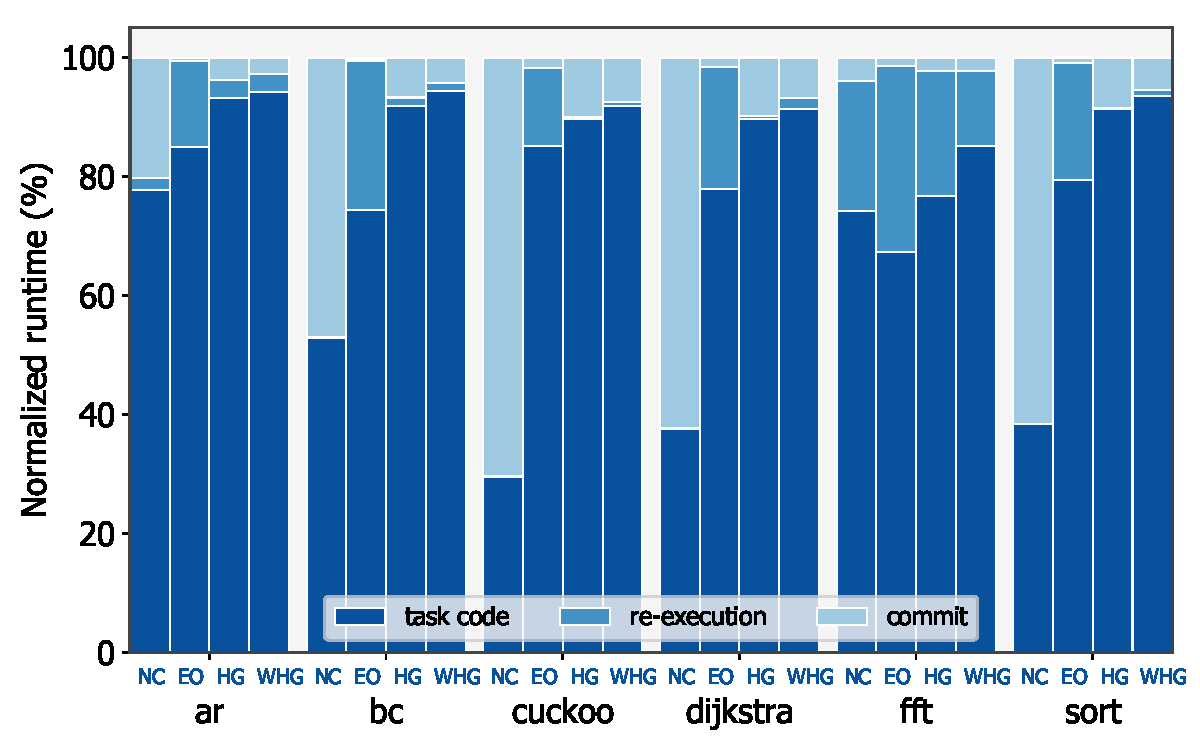
\includegraphics[width=0.5\columnwidth]{figures/coalEfficiency}
	\caption{Normalized \sys time usage for all coalescing strategies compared to non-coalesced \sys with overall \sys overhead breakdown; NC: no coalescing, EB: energy-blind coalescing, EA: energy-aware coalescing, ETA: energy and task-aware coalescing. All \sys coalescing strategies significantly reduce the overhead of (task) commits. EA and ETA perform much better than EB a they reduce re-execution further. \todo{replace user code with task code; increase font by two more points everywhere}{Amjad}}
	\label{fig:overallOverheadBreakdown}
	%\end{figure}
\end{wrapfigure}

Our results illustrate key findings about \sys. We show through extensive qualitative and quantitative evaluation that (i) \sys \emph{provides computation progress} at the partial task level, guaranteeing execution at the worst intermittent energy conditions where state-of-the-art runtimes fail; (ii) usually \emph{improve execution speed} of applications compared to the state-of-the-art runtimes; (iii) \sys through coalescing mechanism \emph{reduces the memory protection overhead} significantly; and (iv) that \sys is \emph{more generic to use} and allows to interact with code written for non-intermittent devices much easier. 

\textbf{Key Performance Indicators.} Our aim is to assess \sys as detailed as possible. For this we have characterized \sys runtime performance (execution time), based on a set of benchmarks, considering core task adaptation mechanisms of \sys: \emph{task coalescing} and \emph{task downscaling}. We also characterize \sys overhead showing precisely what is the source of \sys superior performance investigating task re-execution and commit penalty and memory page access patterns.

We remind the reader that \sys is compared to Alpaca runtime and the benchmarks for Alpaca were hand-transformed in a time-consuming manual process from Clang (LLVM-generated code) to GCC (see Section~\ref{sec:implementation}). The manual code transformation was required as \sys was written with GCC in mind, and Alpaca cannot support any other complier than LLVM.

%Then, we need to know how many tasks \sys can coalesce within a given execution scenario. We ran a subset of applications (split by tasks manually) with continuous power supply and measured the size of tasks for each application and the amount of tasks coalesced. Result is given in Table~\ref{tab:aveVirtuTaskSize}. We see clearly that \sys manages to coalesce more tasks as individual tasks are small. As the size of individual task increases, e.g., as in the case of dft application, the number of coalesced tasks is also small. This result clearly shows that for the benefit of coalescing and for code portability, initial code should be split by \emph{as small tasks as possible}. This will help \sys to find the best possible virtual task size to minimise its runtime.

\subsection{Characterization of \sys Overhead}
\label{sec:coala_overhead}

We start with the assessment of \sys Overhead for all benchmarks. This will lead us to the selection of the best set of coalescing strategies to proceed with.

\indent \textbf{\sys Coalescing Algorithm Efficiency.} We have measured the time spent on executing (i) user code, (ii) task re-execution and (iii) task commits for all coalescing strategies (EB, EA, and ETA) and all benchmarks. We compared our results to non-coalescing \sys (NC). The experiment was performed at 15\,cm WISP to RF generator antenna distance and normalized per benchmark. All benchmarks were using a 256\,B memory page size except for \textbf{bc} which was using 16\,B page. Those page sizes were selected for a large set of potential page sizes and were found to maximize the performance of the respective benchmark. Detailed investigation of \sys paging performance will be given in Section~\ref{sec:results_memory_management}.

The result is presented in Figure~\ref{fig:overallOverheadBreakdown}. We clearly see that any \sys coalescing strategy reduces the cost of task commit for \emph{all} benchmarks. EA and ETA strategies reduce the re-execution cost of tasks further. For this reason we proceed with the investigation of \sys without considering EB coalescing.

\textbf{Overall \sys Overhead Breakdown.} We now proceed with investigating how \sys manipulates task commits: task transitions and memory accesses (including breakdown per SRAM and FRAM access). The result for all benchmarks are measured in the same way as for the results presented earlier (i.e. given in Figure~\ref{fig:overallOverheadBreakdown}) and using the same page sizes as in the earlier experiment. The result is presented in Figure~\ref{fig:coalEfficiency}.

\begin{figure}
	\centering
	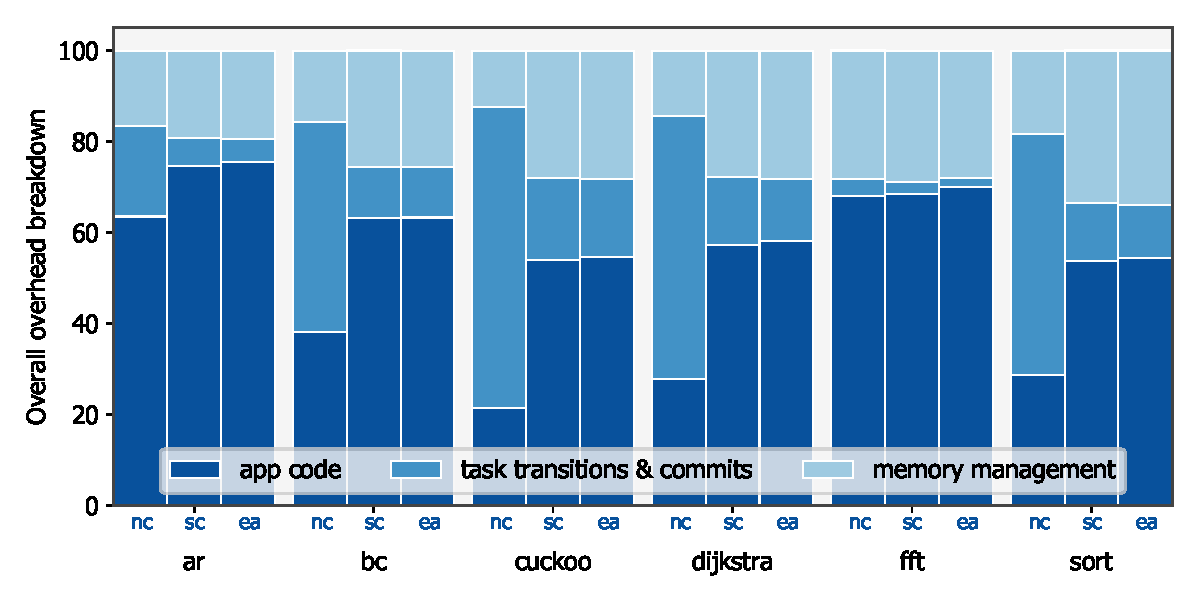
\includegraphics[width=0.49\columnwidth]{figures/overallOverhead}
	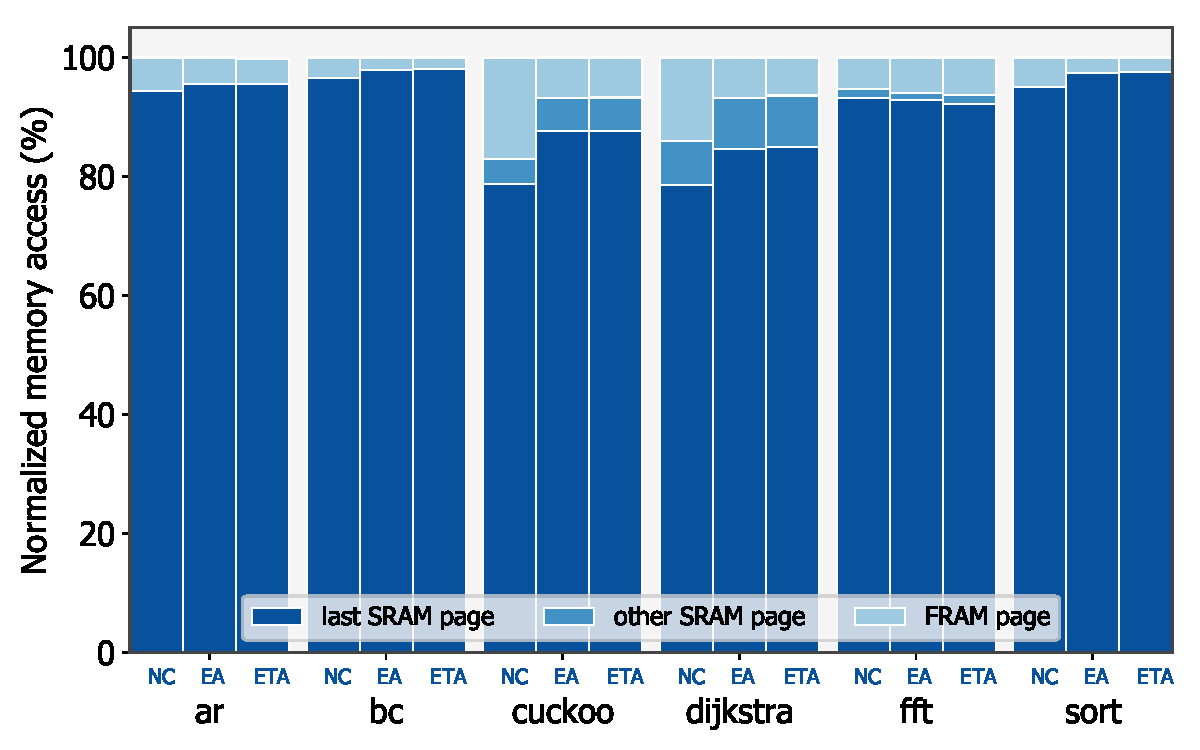
\includegraphics[width=0.49\columnwidth]{figures/memAccess}
	\caption{\sys coalescing algorithm efficiency. Left: load split per task manipulation step; right: detailed breakdown of memory access presented in the left figure); NC: no coalescing, EA: energy-aware coalescing, ETA: energy and task-aware coalescing. \todo{Check if Y axis names are correct; replace task code with user code}{Amjad, Carlo}}
	\label{fig:coalEfficiency}
\end{figure}

Looking into Figure~\ref{fig:coalEfficiency} (left) we see that no coalescing (NC) \sys has a huge cost of task transitions and commits (which recapitulates the result presented in Figure~\ref{fig:overallOverheadBreakdown}). For both coalescing strategies (EA and ETA) memory access constitutes about 30\% of the whole \sys runtime across all benchmarks.

\textbf{\sys Memory Access Overhead Breakdown.} Let us now look into the results on the \sys memory operation process, i.e. we will show specifically which parts of memory from Figure~
\ref{fig:coalEfficiency} (left) are accessed. The result is presented in Figure~\ref{fig:coalEfficiency} (right). We immediately see that majority of operations are targeting the last SRAM page and very little operations on the FRAM pages. There are very few operations involving other SRAM pages than the last one (only visible for \textbf{cuckoo} and \textbf{dijkstra}). 

\subsection{\sys Task Adaptation}
\label{sec:result_coalescing}

We characterize \sys by studying how its execution time varies due to task adaptation. We look at \sys in isolation and in comparison to Alpaca.

\textbf{\sys Coalescing Execution Time.}  Figure~\ref{fig:coalescing} shows the run time of \sys's three coalescing strategies for all benchmarks normalized to the \sys runtime without coalescing. We show data from experiments measured in the same was as for the results in Section~\ref{sec:coala_overhead}. 

The result in Figure~\ref{fig:coalescing} recapitulates the result presented in Figure~\ref{fig:overallOverheadBreakdown} showing the benefit in \emph {normalized runtime} from coalescing (for EA and ETA case) for all applications compared to non-coalescing (NC) case. Coalescing improves \sys's performance by eliminating the overhead of committing after each task. The difference in performance between coalescing and no coalescing is, however, highly application-dependent. Then, the gain from energy and task-aware strategy (ETA) compared to energy-aware only (EA) are almost non-existent for applications, except for \textbf{fft}, i.e. the one with with large tasks. Furthermore, the \textbf{cuckoo} application (like other top-performers, \textbf{bc} and \textbf{sort}) has small tasks that \sys can easily coalesce to eliminate many commits.

\begin{wrapfigure}{t!}{0.5\textwidth}
%\begin{figure}
	\centering
	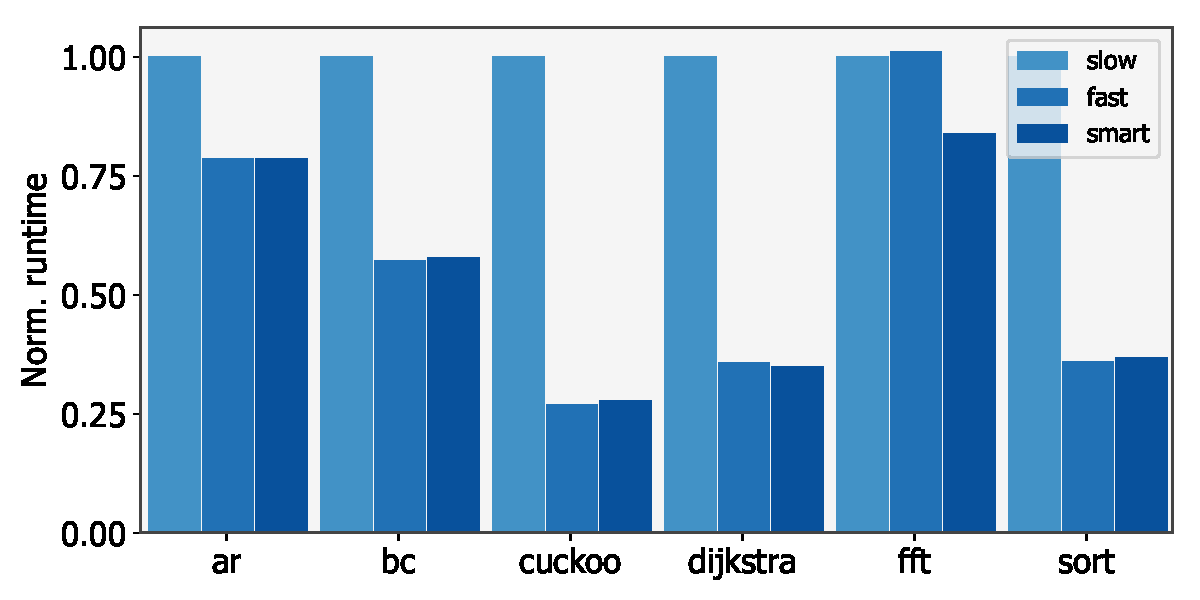
\includegraphics[width=0.5\columnwidth]{figures/coalStrategies}
	\caption{\sys coalescing strategies (EA and ETA) performance per application on intermittent power (RF generator at 15\,cm from the WISP) compared to \sys without coalescing (NC). \sys task coalescing strategy provides significant improvements (from 0.25, \textbf{ar}, up to 0.70, \textbf{sort}) compared to a non-coalesced system.}
	\label{fig:coalescing}
%\end{figure} 
\end{wrapfigure}

\textbf{\sys versus non-adaptive Task-based Model.} We now evaluate \sys's run time performance and compare \sys to the performance of Alpaca runtime, i.e. a non-adaptive task-based system. Results are presented in Figure~\ref{fig:runtime}. For each application we measured its execution time using real wireless power provisioned from the RF signal generator at three distances (refer again to Section~\ref{sec:implementation}).

\begin{wrapfigure}{t!}{0.5\textwidth}
%\begin{figure}
	\centering
	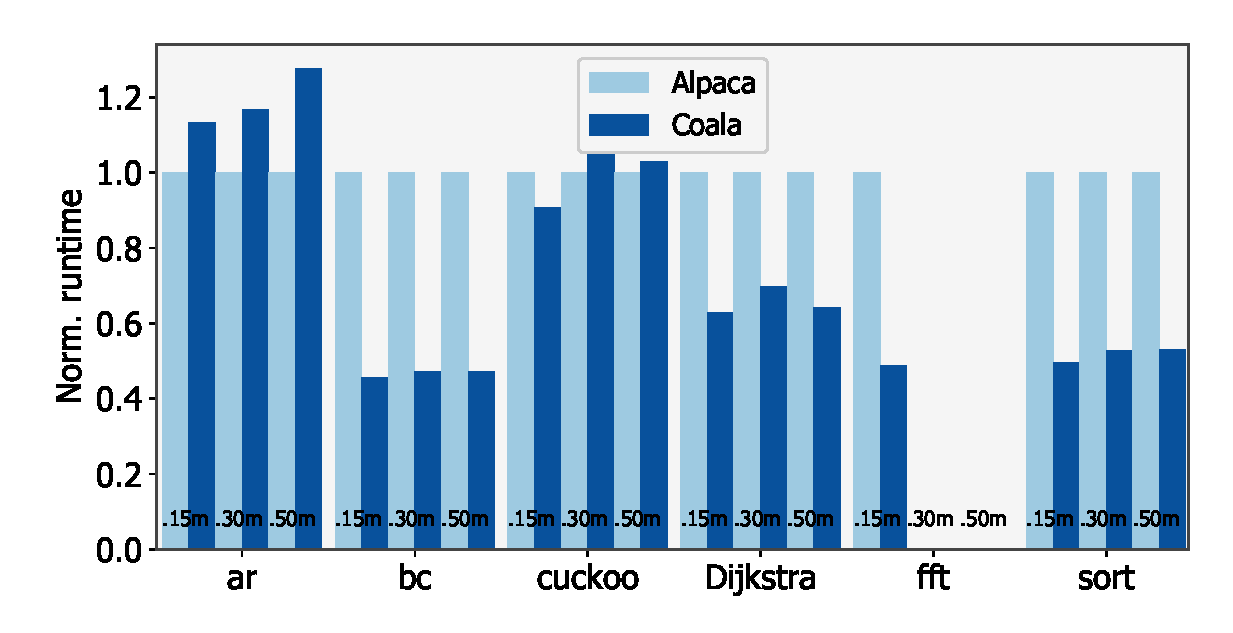
\includegraphics[width=0.5\columnwidth]{figures/coala_alpaca_gcc}
	\caption{Performance of \sys applications at multiple WISP to RF generator antenna distances \{0.15, 0.3, 0.5\}\,m (left, center and right-most bar per application, respectively), compared against Alpaca (results normalized) for ETA coalescing strategy. Results show that \sys performs on average better than Alpaca for majority of the benchmarks. For specific benchmarks \sys performs worse than Alpaca \todo{state why it is sometimes worse}{Carlo}}
	\label{fig:runtime}
%\end{figure}
\end{wrapfigure}

The data show the average execution time of each application with runtimes normalized to \sys's average. \todo{verify this statement}{Przemek} The results show that \sys provides a performance benefit compared to Alpaca for most applications (all except for \textbf{ar} and \textbf{cuckoo}). The performance benefit is the greatest for applications that perform repeating read and write operations, particularly if involving arrays (\textbf{bc}, \textbf{sort}, \textbf{dijkstra}). This effect is seen at all distances on intermittent power. In applications with protected variables (or array elements) accessed next to each other but residing in different SRAM or FRAM pages \sys incurs overhead from memory virtualization that cause its performance to be comparable to (or worse than) Alpaca (\textbf{ar}, \textbf{dijkstra}). 

Another critical observation is that \textbf{fft} benchmark did not complete at any distance larger than 0.15\,cm. As we will show now, \sys task downscaling mechanism will be able to solve this issue.  

\textbf{Task Downscaling Execution Time.} We have enabled task downscaling and measured the execution time for \textbf{fft} benchmark at all distances that this benchmark could not execute (refer again to Figure~\ref{fig:coalescing} and $\infty$ marks). \sys could execute the benchmark successfully with the execution time of X\,s at a distances of $d= 0.6$\,m, i.e. the one that exceeds the furthest distance ($d=0.5$\,m) presented in Figure~\ref{fig:runtime}, respectively.

\subsection{\sys Paging Performance}
\label{sec:results_memory_management}

We have also evaluated the effect that paging with different page sizes has on \sys's performance. We show data in Figure~\ref{fig:page_size}; The left plot shows the run time performance normalized to the best per-application performance, using pages of different sizes in \sys; the right plot shows the number of page faults for the same set of executions normalized to the maximum of each set. We measured performance as MCU clock cycles using values read out by TI's Code Composer Studio IDE. 

\textbf{Effect of Page Size on \sys Runtime.} The results (Figure~\ref{fig:page_size}, left) show a ``bathtub curve'' in the performance of each application (the effect would be more profound with a larger set of pages than we considered), as the number of page faults varies. The data show that across application there is a page size that minimizes \emph{both} execution time. We observe that the page size is not the same for each application, although 128\,B pages perform well for all applications. 

\textbf{Page Size versus Page Faults in \sys Runtime.} The increased rate of page faults (Figure~\ref{fig:page_size}, right) is responsible for the overhead with small page sizes; smaller pages require accessing more different pages, leading to higher paging costs. With larger page sizes, the overhead is higher than with moderate pages, too. The explanation for these higher overheads is that large pages have a higher commit cost. Even if an application accesses few memory locations, \sys pages data at full page size, degrading performance by sometimes paging in and out unnecessary data. The data reveal a reasonable default page size of 128\,B and when developing an application, a programmer should consider varying the page size to moderate poor performance.

\begin{figure}
	\centering
	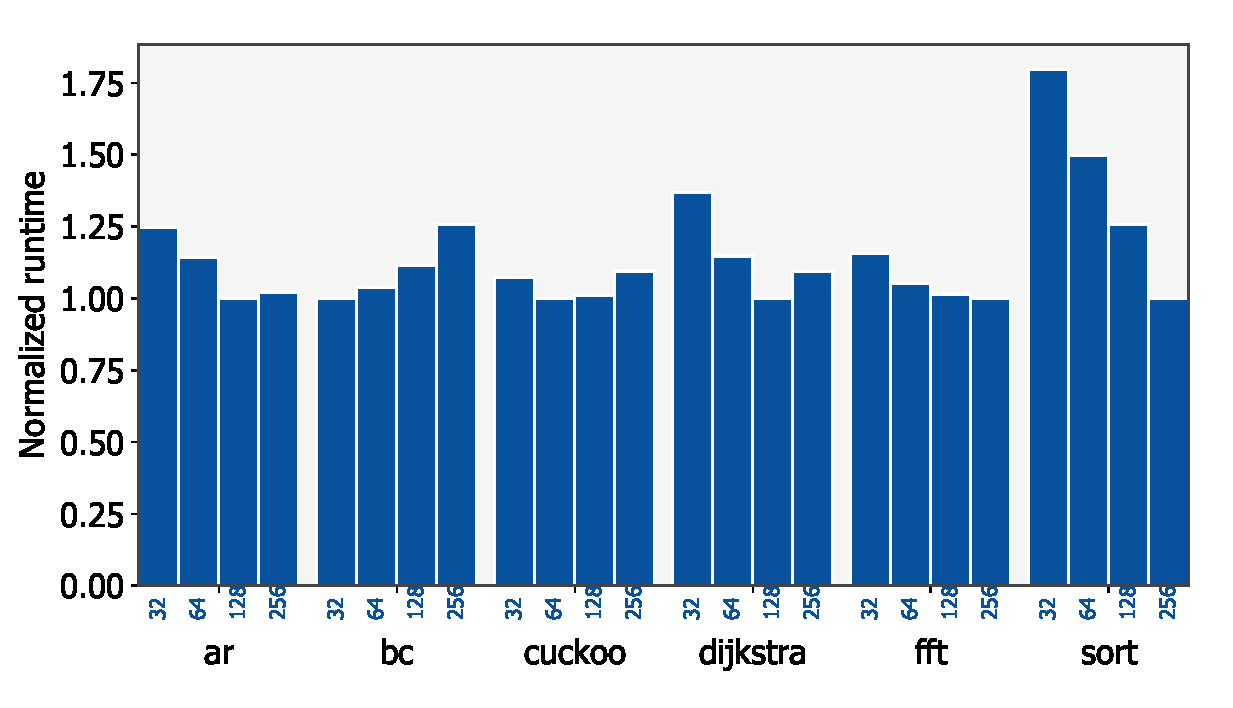
\includegraphics[width=0.49\columnwidth]{figures/page_exec-time}
	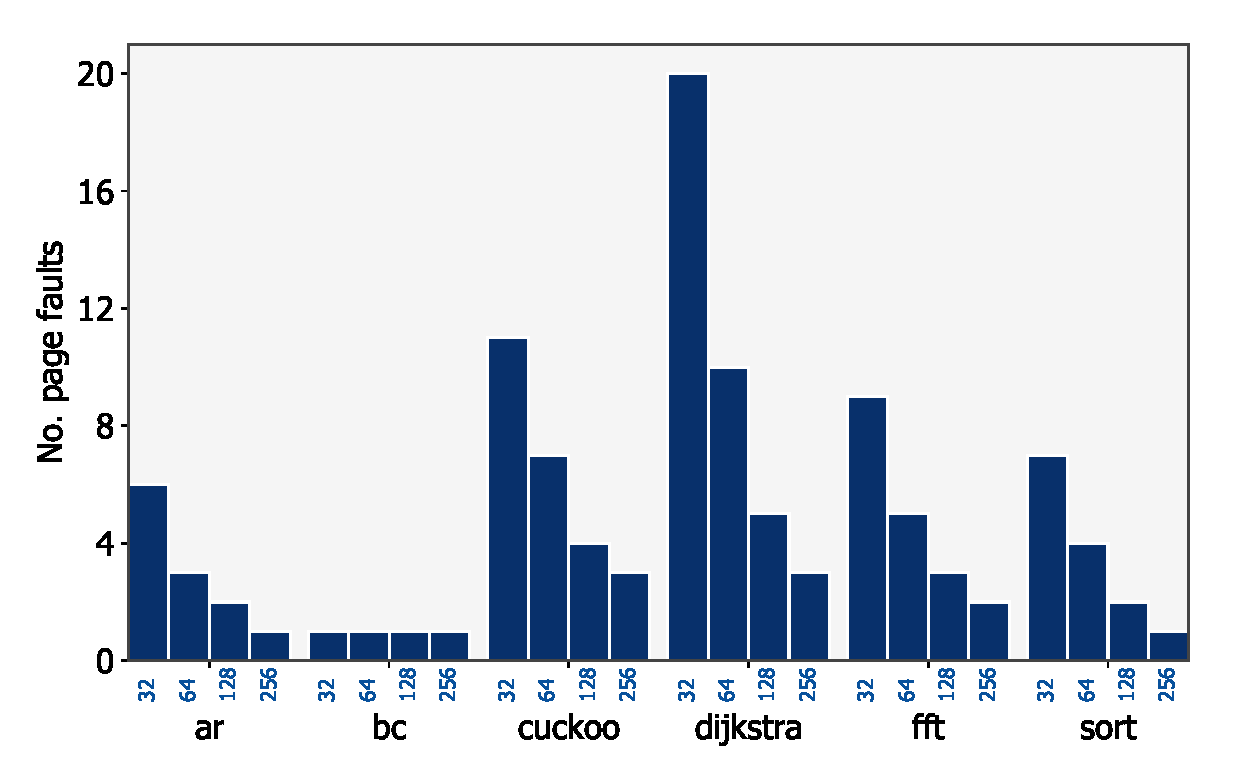
\includegraphics[width=0.49\columnwidth]{figures/pagePulls}
	\caption{\sys normalized runtime for various page sizes, \{32, 64,128,256\}\,B (left) and respective page pulls (bottom) for all benchmarks.}
	\label{fig:page_size}
\end{figure}

%\subsection{\sys Memory Footprint?}
%\label{sec:results_program_characterization}
%
%\begin{table}
%	\begin{tabular}{| c | c | c | c | c |}
%		\hline
%		\multirow{2}{*}{Application} & \multicolumn{2}{ c |}{Memory footprint} & \multirow{2}{*}{No. tasks} & \multirow{2}{*}{SLOC} \\
%		\cline{2-3}
%		{} & \sys & Alpaca & {} & {} \\
%		\hline\hline
%				\textbf{ar} & --- & --- & --- & ---\\
%		\hline
%				\textbf{bc} & --- & --- & --- & ---\\
%		\hline
%				\textbf{cuckoo} & --- & --- & --- & ---\\
%		\hline
%				\textbf{dijkstra} & --- & --- & --- & ---\\
%		\hline
%				\textbf{fft} & --- & --- & --- & ---\\
%		\hline
%				\textbf{sort} & --- & --- & --- & ---\\
%		\hline
%	\end{tabular}
%		\caption{Comparison between \sys and Alpaca benchmarks.}
%		\label{table:compiler_result}\vspace{-0.5cm}
%\end{table}

%\begin{table}[t]
%	\centering
%	\renewcommand{\tabcolsep}{1pt}
%	\begin{tabular}{|l|cc|cc|cc|cc|c|}
%		\hline
%		{} & \multicolumn{2}{c|}{{\bf Prot. bytes}} & \multicolumn{2}{c|}{{\bf \# Tasks}} & \multicolumn{2}{c|}{{\bf \# Prot. acc.}} & \multicolumn{2}{c|}{\bf SLOC} & {\bf Comp.} \\
%		App & Man. & Comp. & Man. & Comp. & Man. & Comp. & \multicolumn{1}{l}{\sys} & \multicolumn{1}{r|}{Chain~\cite{chain}} & {\bf time} \\
%		\hline\hline
%		bc & 22 & 22 & 10 & 15 & 81 & 93 & 351 &588 & 3\\
%		cem & 3492 & 3242 & 12 & 9 & 92 & 123 & 388 &721 & 2\\
%		cuckoo & 282 & 288 & 15 & 6 & 90 & 76 & 483 &762 & 6\\
%		rsa & 332 & 250 & 20 & 27 & 130 & 296 & 887 &1233 & 86\\
%		ar & 166 & 218 & 11 & 6 & 112 & 333 & 483 &762 & 34\\
%		sort & 104 & 104 & 4 & 2 & 70 & 23 & 180 & 287 & $<$1\\
%		dft$^\dagger$ & --- & --- & --- & --- & --- & --- & 222 & 293 & ---\\
%		%dd &  &  &  &  &  &  &  & 287 &  \\
%		\hline
%	\end{tabular}
%		\caption{Comparison between \sys and Alpaca benchmarks.}
%		\label{table:compiler_result}\vspace{-0.5cm}
%\end{table}
